\documentclass[letterpaper,11pt]{article}
\oddsidemargin -1.0cm \textwidth 17.5cm

\usepackage[utf8]{inputenc}
\usepackage[activeacute,spanish, es-lcroman]{babel}
\decimalpoint
\usepackage{amsfonts,setspace}
\usepackage{amsmath}
\usepackage{amssymb, amsmath, amsthm}
\usepackage{comment}
\usepackage{float}
\usepackage{amssymb}
\usepackage{dsfont}
\usepackage{anysize}
\usepackage{multicol}
\usepackage{enumerate}
\usepackage{graphicx}
\usepackage[left=1.5cm,top=2cm,right=1.5cm, bottom=1.7cm]{geometry}
\setlength\headheight{1.5em} 
\usepackage{fancyhdr}
\usepackage{multicol}
\usepackage{hyperref}
\usepackage{wrapfig}
\usepackage{subcaption}
\usepackage{siunitx}
\usepackage{cancel}
\usepackage{mdwlist}
\usepackage{svg}
\pagestyle{fancy}
\fancyhf{}
\renewcommand{\labelenumi}{\normalsize\bfseries P\arabic{enumi}.}
\renewcommand{\labelenumii}{\normalsize\bfseries (\alph{enumii})}
\renewcommand{\labelenumiii}{\normalsize\bfseries \roman{enumiii})}

\begin{document}
\graphicspath{{../2020-1/}}  % pa que compile las imágenes

\fancyhead[L]{\itshape{Facultad de Ciencias F\'isicas y Matem\'aticas}}
\fancyhead[R]{\itshape{Universidad de Chile}}

% \begin{minipage}{11.5cm}
%     \begin{flushleft}
%         \hspace*{-0.6cm}\textbf{FI1000-1 Introducción a la Física Clásica}\\
%         \hspace*{-0.6cm}\textbf{Profesor:} Ignacio Bordeu\\
%         \hspace*{-0.6cm}\textbf{Auxiliares:} Alejandro Cartes \& Simón Yáñez\\
%         \hspace*{-0.6cm}\textbf{Ayudante:} Javier Cubillos\\
%     \end{flushleft}
% \end{minipage}

\begin{center}
	\LARGE \textbf{Resumen Trigonometría}\\ %posible resumen
	\small{Alejandro Cartes\\
	\small{\href{mailto:alejandroml.cartes@gmail.com}{mail: alejandroml.cartes@gmail.com}}}
\end{center}

\begin{picture}(2,3)
    \svgpath{../2021-2}  % descomentar si se agrega a carpeta "auxiliares"
    \put(415, 35){\includesvg[scale=0.23]{img/dfi.svg}}
\end{picture}

\rfoot[]{pág. \thepage}

\section{Definiciones trigonométricas}

Para un triángulo rectángulo se definen las siguientes relaciones entre ángulo y lados: \par
{
\begin{wrapfigure}[5]{l}{0.25\textwidth}
    \centering
    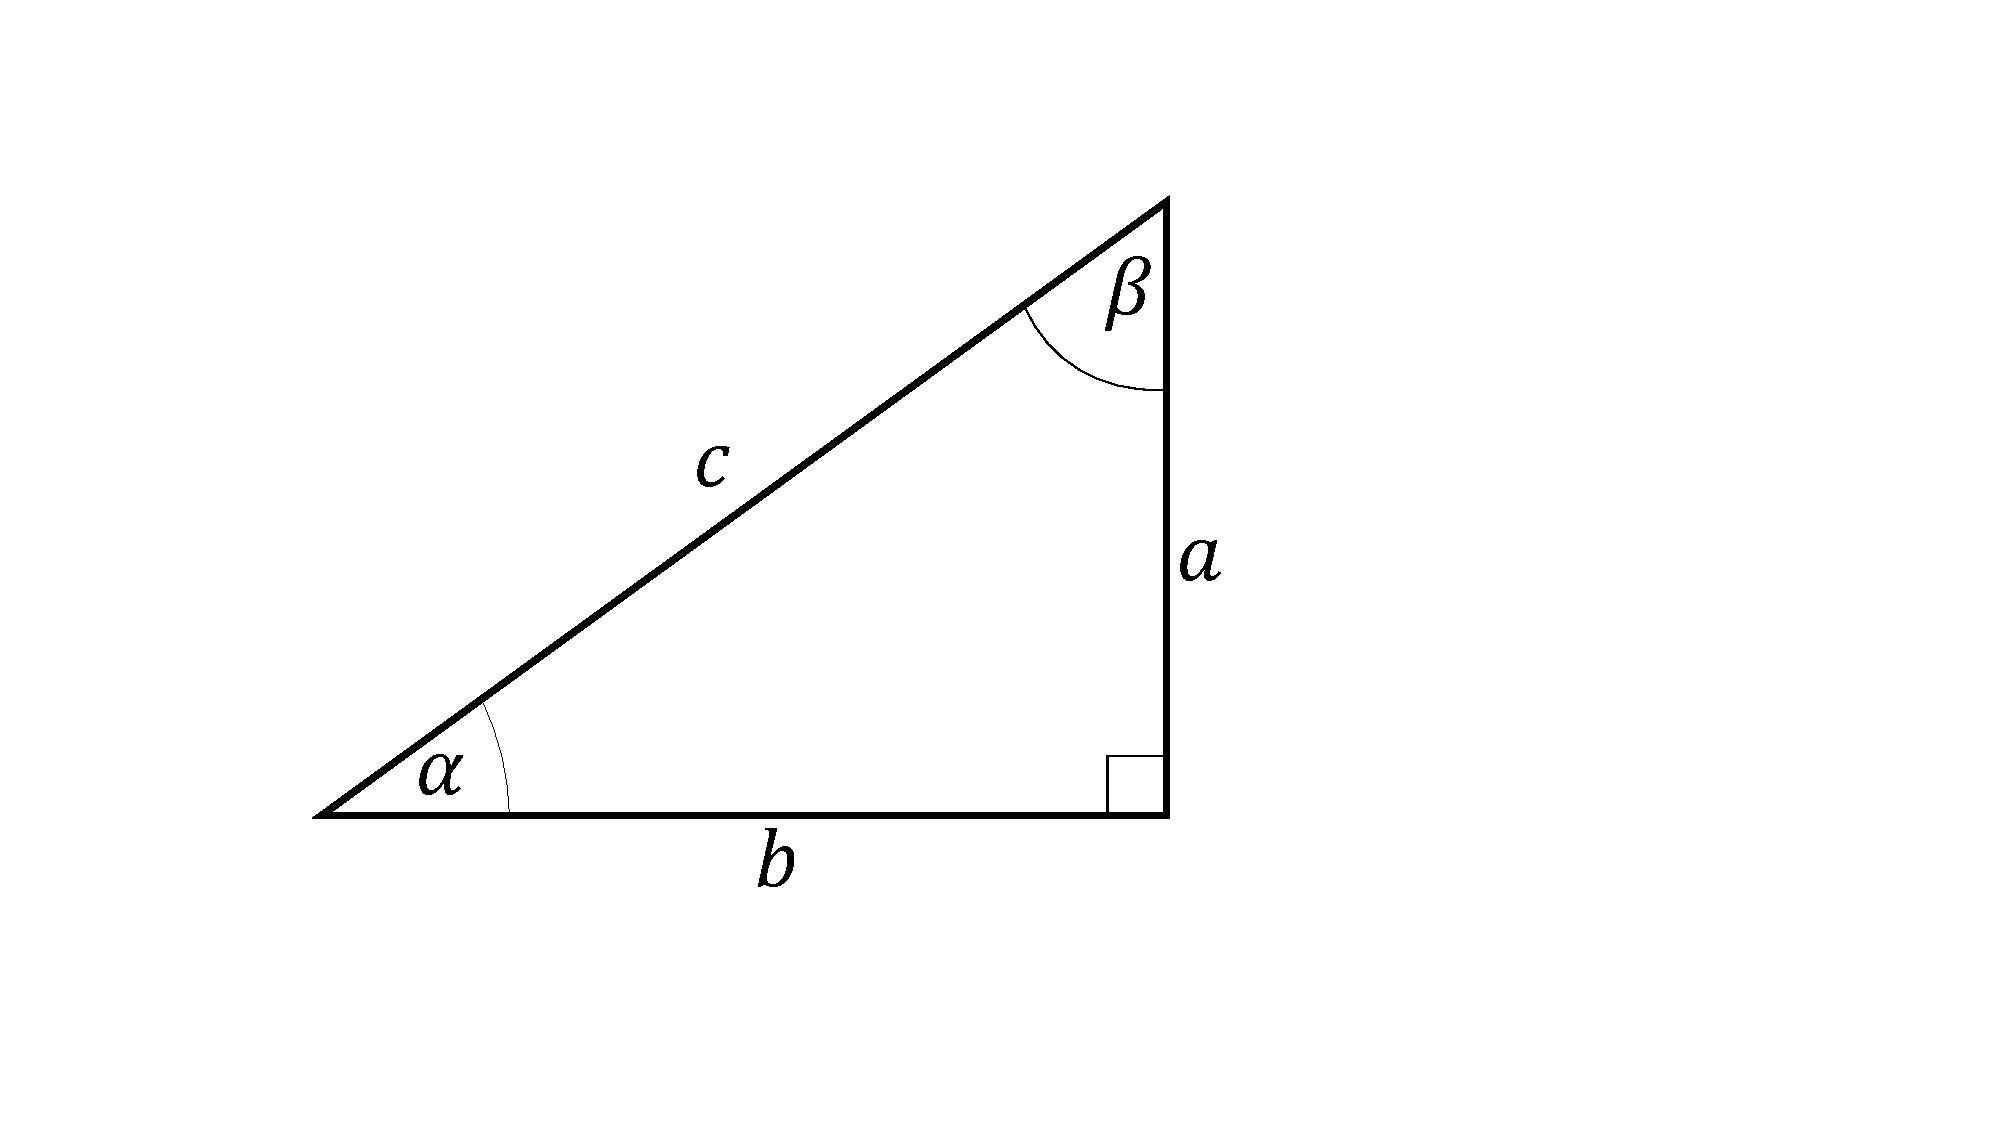
\includegraphics[scale=0.30]{Imágenes/resumen trig/triang.pdf}  
\end{wrapfigure}
\begin{align*}
    \sin\alpha&=\frac{a}{c}=\frac{\text{cat. opuesto}}{\text{hipotenusa}} &  \csc\alpha&=\frac{1}{\sin\alpha}=\frac{c}{a}\\
    \cos\alpha&=\frac{b}{c}=\frac{\text{cat. adyacente}}{\text{hipotenusa}}  & \sec\alpha&=\frac{1}{\cos\alpha}=\frac{c}{b}\\
    \tan\alpha&=\frac{a}{b}=\frac{\text{cat. opuesto}}{\text{cat. adyacente}}=\frac{\sin\alpha}{\cos\alpha} & \cot\alpha&=\frac{1}{\tan\alpha}=\frac{b}{a}
\end{align*}
}

\section{Ángulos y Radianes}{
\begin{wrapfigure}[6]{R}{6cm}
\end{wrapfigure}
\begin{picture}(2,3)
    \put(330,-120){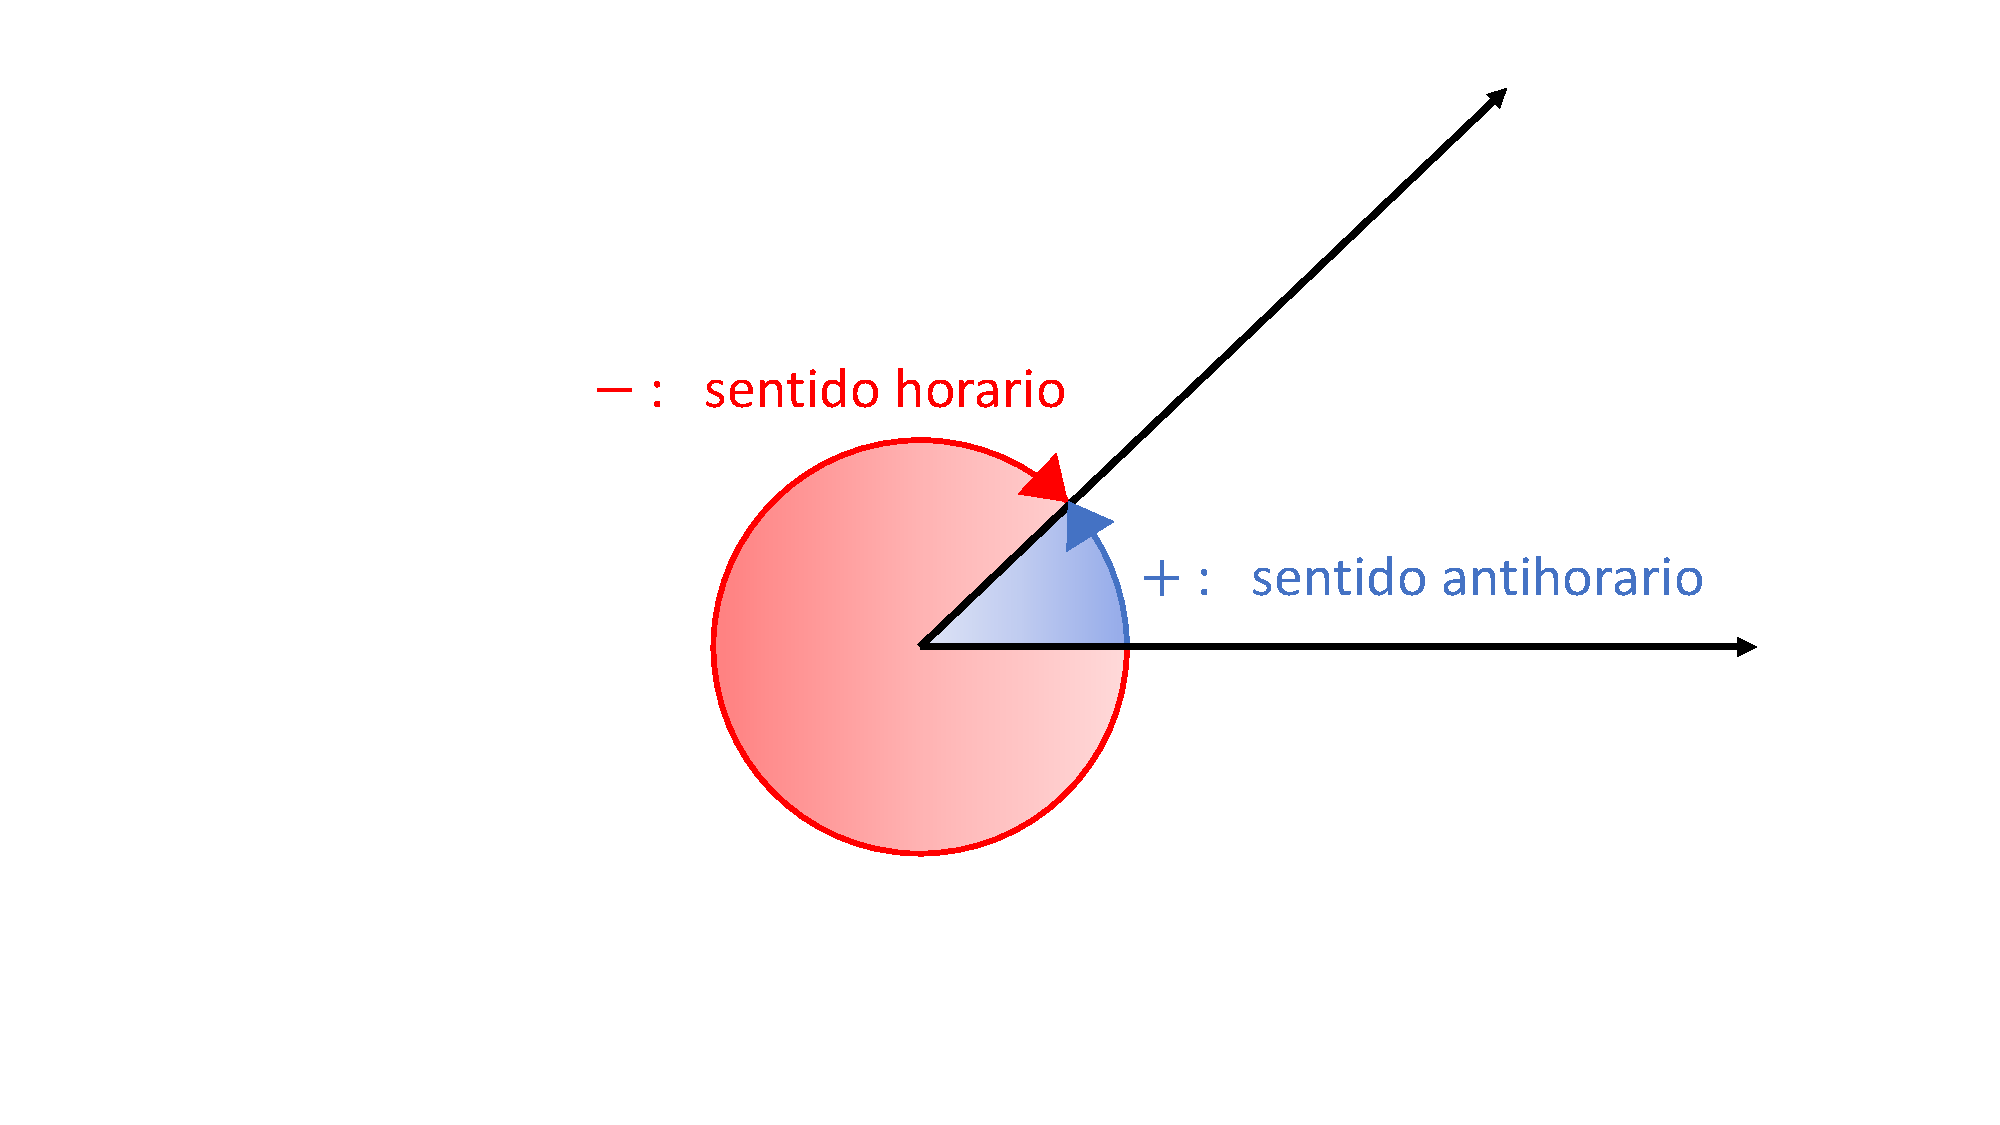
\includegraphics[scale=0.25]{Imágenes/resumen trig/ang.pdf}}
\end{picture}

Se denomina ángulo a la sección del plano que queda comprendida entre dos semirrectas que se originan en un mismo punto, y están colocadas en distintas direcciones.\\
Se define que un ángulo es \textbf{positivo} cuando se mide en el sentido \textbf{antihorario} (contrario a las agujas del reloj), y por
lo tanto es \textbf{negativo} si se mide en sentido contrario, es decir, en el sentido \textbf{horario} (mismo que las agujas del reloj).\par
}

Existen distintos sistemas de medición de ángulos (de manera análoga a la que existen distintos sistemas para medir, por ejemplo, distancias: millas, kilómetros, leguas, etc.). El sistema más conocido es el  \textbf{sistema sexagesimal} el cual mide los ángulos en \textbf{grados, minutos y segundos} ($1^{\circ}\equiv 60^{\prime}$ y $1^{\prime}\equiv60^{\prime\prime}$), donde una vuelta a la circunferencia corresponde a $360^{\circ}$.\\
De ahora en adelante nos centraremos en el \textbf{sistema circular} el cual mide los ángulos en \textbf{radianes}, donde una vuelta a la circunferencia corresponde a $2\pi [rad]$ o simplemente $2\pi$.

\subsection*{¿Qué es un radián?}

Para definir un radián, primero consideremos una longitud de arco $L$. Con una simple regla de tres, se tiene que: \par
{
\begin{wrapfigure}[10]{l}{5cm}
    \centering
    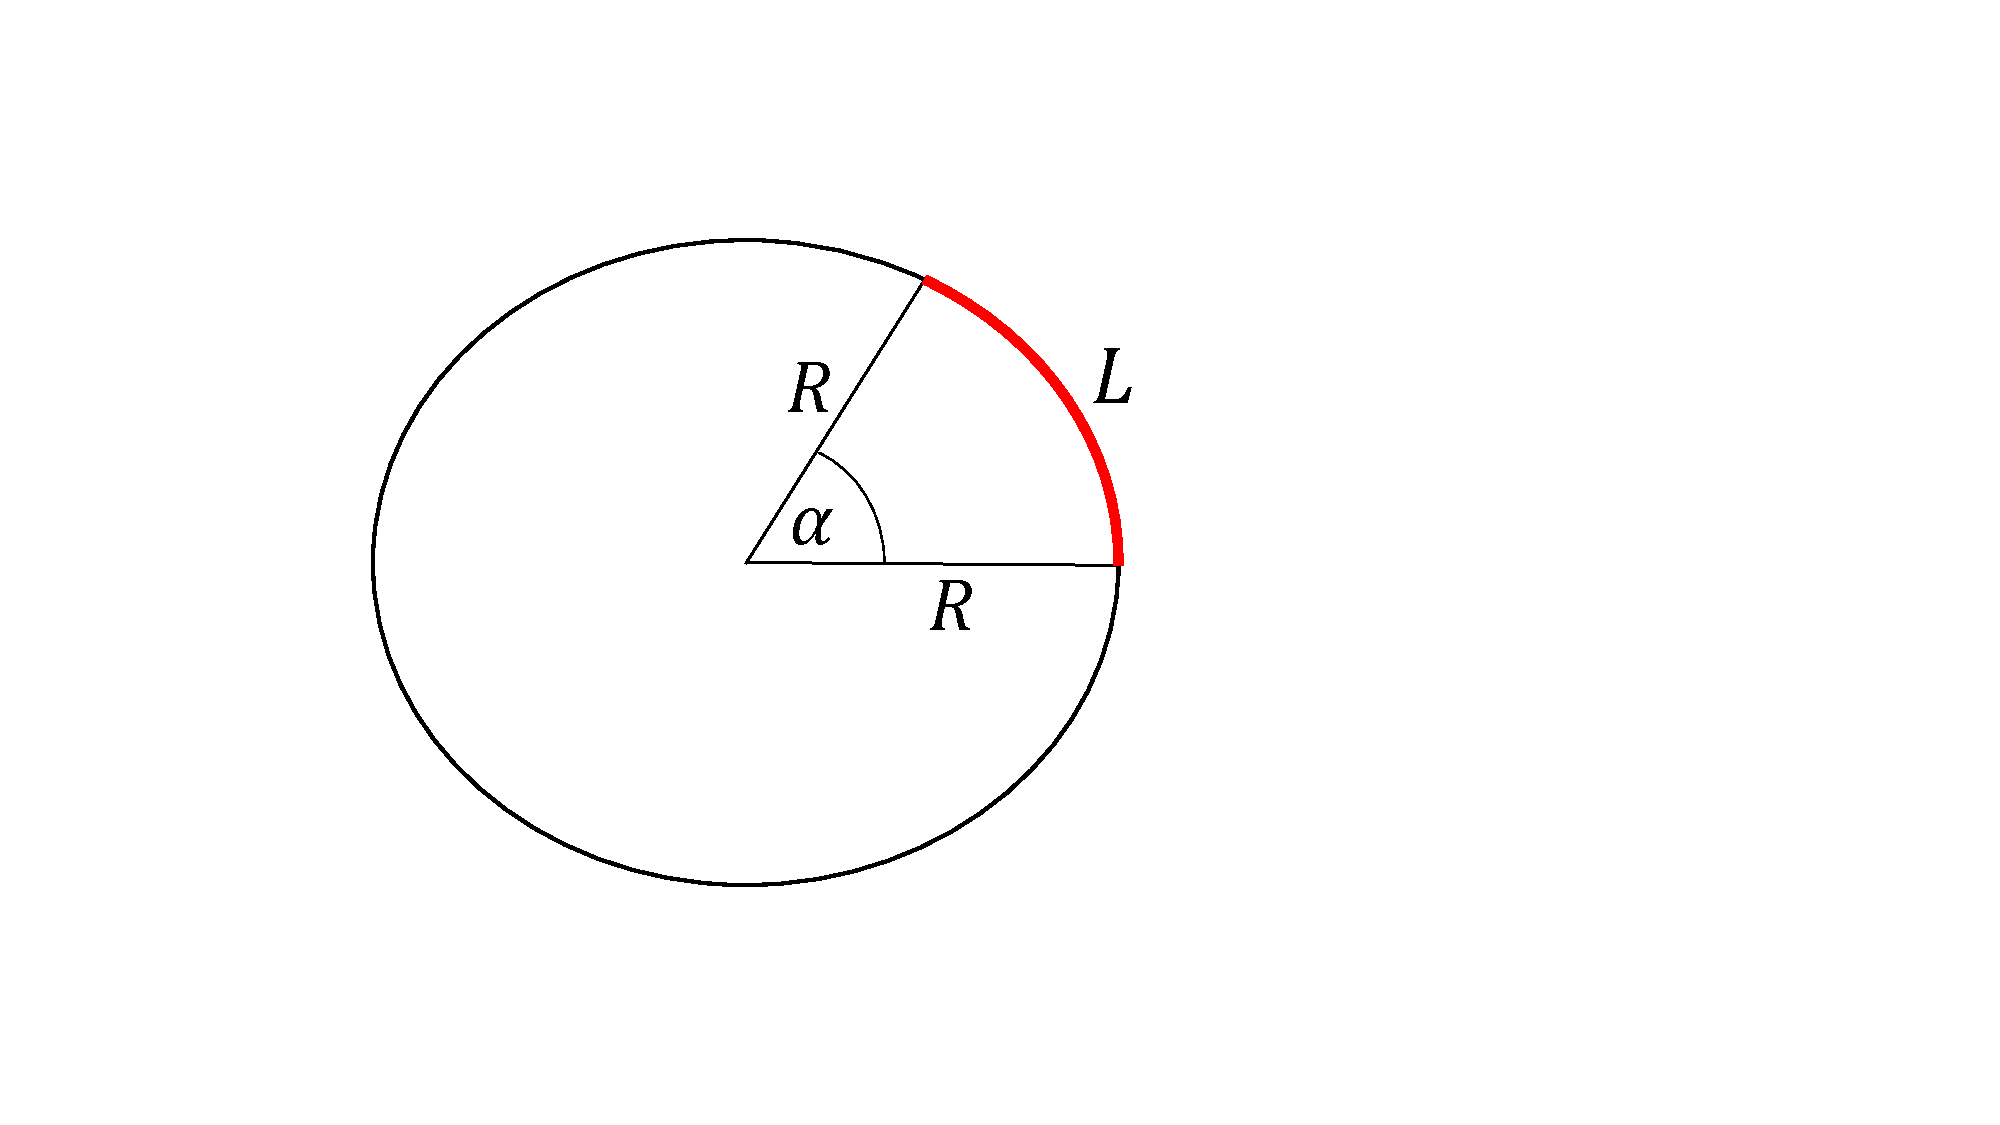
\includegraphics[scale=0.30]{Imágenes/resumen trig/circ.pdf}  
\end{wrapfigure}
\begin{align*}
2\pi [rad] \quad &\longrightarrow \quad 2\pi R \text{  (Perímetro circunferencia)} \\
\alpha \quad & \longrightarrow \quad L\\
\therefore\quad & L=\alpha R
\end{align*}\par
Esto quiere decir que $1 [rad]$ se define como el ángulo para el cual la longitud de arco $L$ es igual al radio $R$ de la circunferencia.\par
}
\newpage
Para pasar de grados a radianes: recordar que $\pi=180^{\circ}$ y realizar una regla de 3:

\begin{table}[h!]
    \centering
    \begin{tabular}{|m{2em}||m{2em}|m{2em}|m{2em}|m{2em}|m{2em}|m{2em}|m{2em}|m{2em}|}
    \hline
    $^{\circ}$ & $0$ & $30$ & $45$ & $60$ & $90$ & $180$ & $270$ & $360$ \\[1ex]\hline
    $rad$ & $0$ & $\cfrac{\pi}{6}$ & $\cfrac{\pi}{4}$ & $\cfrac{\pi}{3}$ & $\cfrac{\pi}{2}$ & $\pi$ & $\cfrac{3\pi}{2}$ & $2\pi$ \\ [3ex] 
    \hline
    \end{tabular}
\end{table}

De esta manera se determina que $1 [rad]=180/\pi\approx 57.296^{\circ}$

\section{Trigonometría en una Circunferencia}
Consideremos una circunferencia de radio $R$ centrada en el origen y un punto cualquiera de esta. Las funciones trigonométricas nos permitirá determinar la \textbf{proyección} del punto en los ejes. Por las definiciones dadas se tiene que:

\begin{figure}[h!]
    \centering
    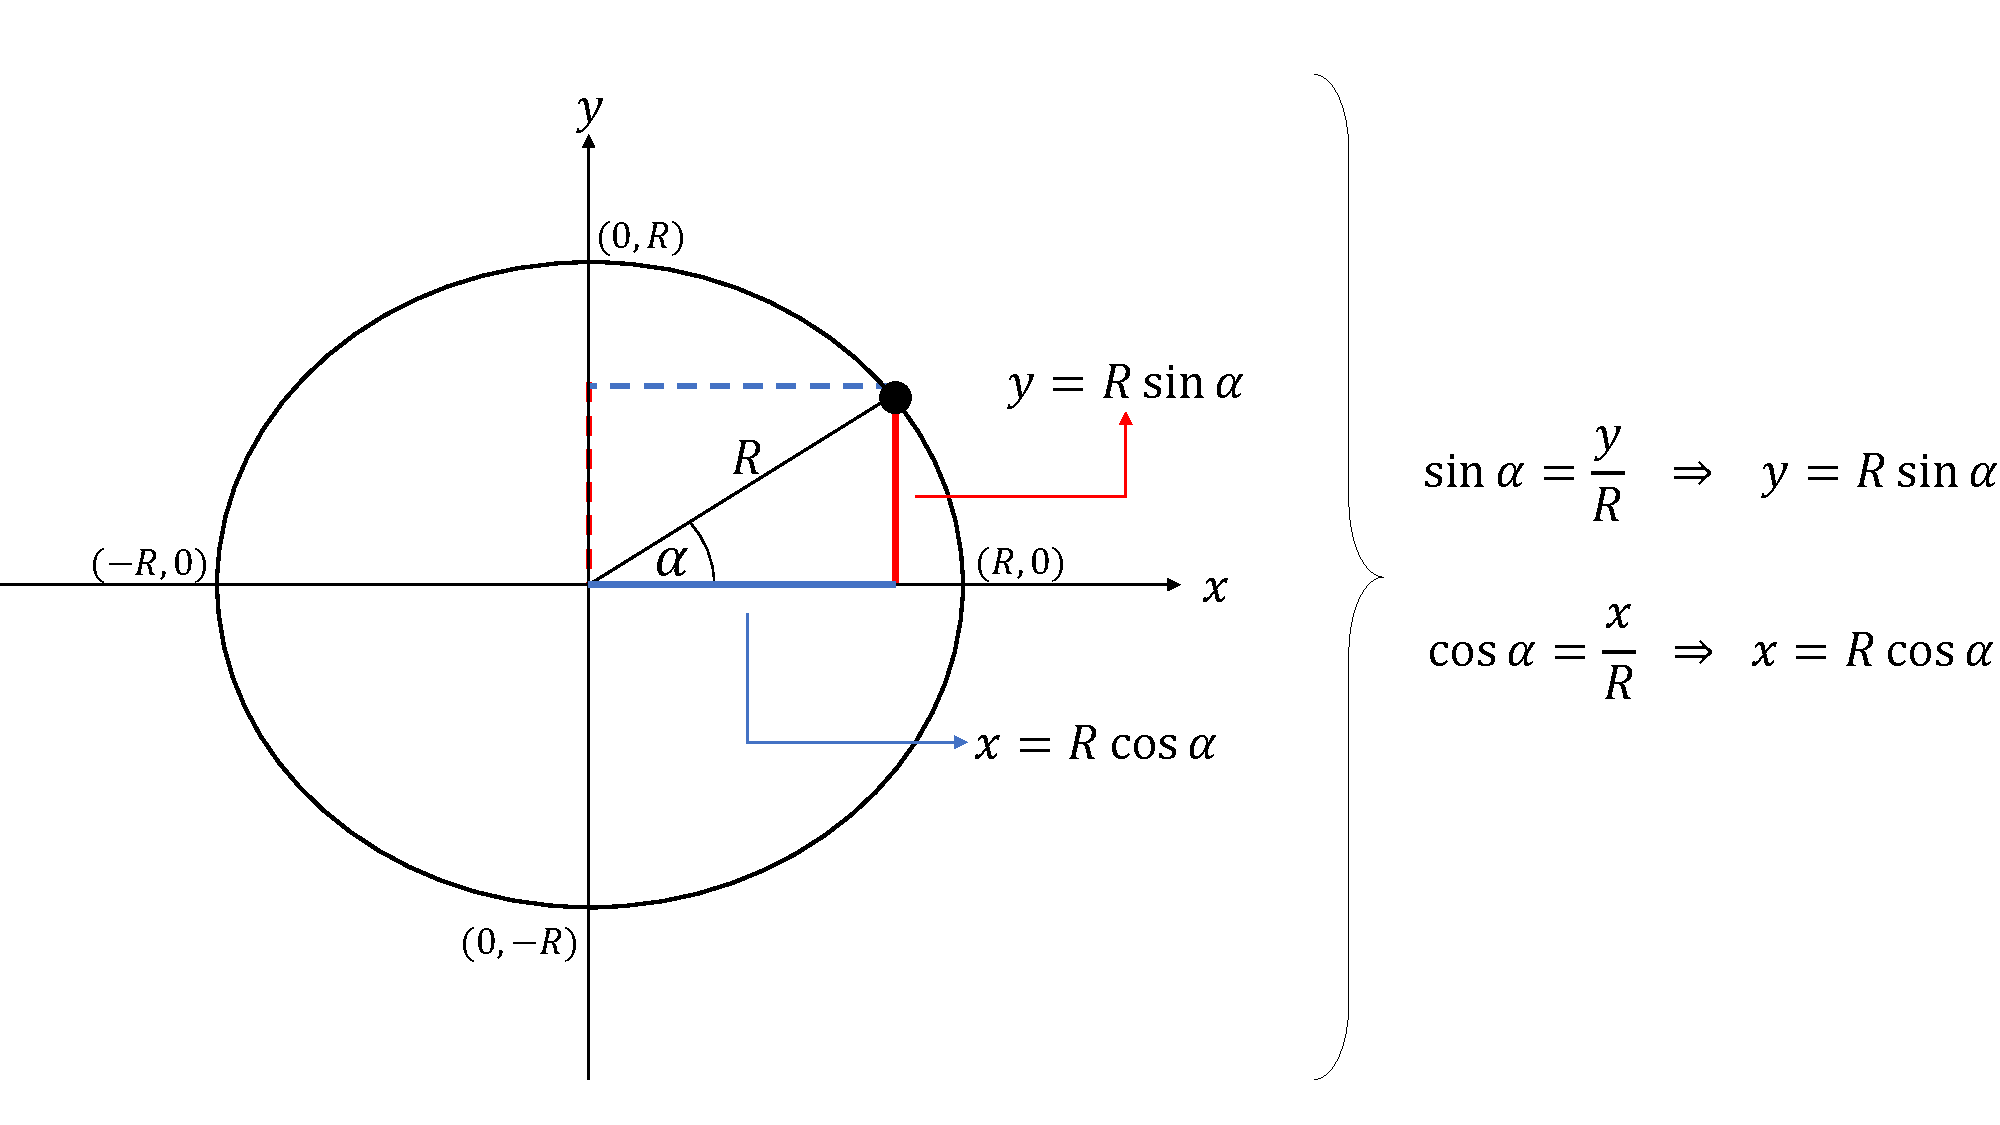
\includegraphics[scale=0.3]{Imágenes/resumen trig/trigcirc.pdf}
\end{figure}

Con esto en mente podemos deducir algunas propiedades muy importantes:

\begin{itemize}
\item Por teorema de Pitágoras se tiene que:

\begin{equation*}
    (R\sin\alpha)^2+(R\cos\alpha)^2=R^2 \quad \Rightarrow \quad \sin^2\alpha+\cos^2\alpha=1
\end{equation*}

\item Algunos valores:
    \begin{itemize}
        \item si $\alpha=0$:
        \begin{itemize}
            \item la proyección en $x$ es máxima y vale $R$, luego $R\cos(0)=R\Rightarrow\cos(0)=1$
            \item la proyección en $y$ es nula, luego $R\sin(0)=0\Rightarrow \sin(0)=0$
        \end{itemize}
        \item si $\alpha=\pi/2$:
        \begin{itemize}
            \item la proyección en $x$ es nula, luego $R\cos(\pi/2)=0 \Rightarrow \cos(\pi/2)=0$
            \item la proyección en $y$ es máxima y vale $R$, luego $R\sin(\pi/2)=R \Rightarrow \sin(\pi/2)=1$
        \end{itemize}
        
        \item si $\alpha=\pi$: 
        \begin{itemize}
            \item la proyección en $x$ es mínima y vale $-R$, luego $R\cos(\pi)=-R \Rightarrow \cos(\pi)=-1$
            \item la proyección en $y$ es nula, luego $R\sin(\pi)=0 \Rightarrow \sin(\pi)=0$
        \end{itemize}
        
        \item si $\alpha=3\pi/2$:
        \begin{itemize}
            \item la proyección en $x$ es nula, luego $R\cos(3\pi/2)=0 \Rightarrow \cos(3\pi/2)=0$
            \item la proyección en $y$ es mínima y vale $-R$, luego $R\sin(3\pi/2)=-R \Rightarrow \sin(3\pi/2)=-1$
        
        \end{itemize}
        
        \item si $\alpha=2\pi$: lo mismo que con $\alpha=0$, pues dimos la vuelta
    \end{itemize}
    Esto nos quiere decir que $-1\leq\cos\alpha\leq1 $ y $-1\leq\sin\alpha\leq1$ para cualquier valor de $\alpha$.
\item Signos:
    \begin{itemize}
        \item si $\alpha \in (0,\pi/2)\text{ }$: $\quad \cos\alpha >0 \quad \sin\alpha>0 \quad \tan\alpha>0$
        
        \item si $\alpha \in (\pi/2,\pi)\text{ }$: $\quad \cos\alpha <0 \quad \sin\alpha>0 \quad \tan\alpha<0$
        
        \item si $\alpha \in (\pi,3\pi/2)$: $\quad \cos\alpha <0 \quad \sin\alpha<0 \quad \tan\alpha>0$
        
        \item si $\alpha \in (3\pi/2,2\pi)$: $\quad \cos\alpha >0 \quad \sin\alpha<0 \quad \tan\alpha<0$
        
    \end{itemize}
    \begin{picture}(2,3)
        \put(330,-20){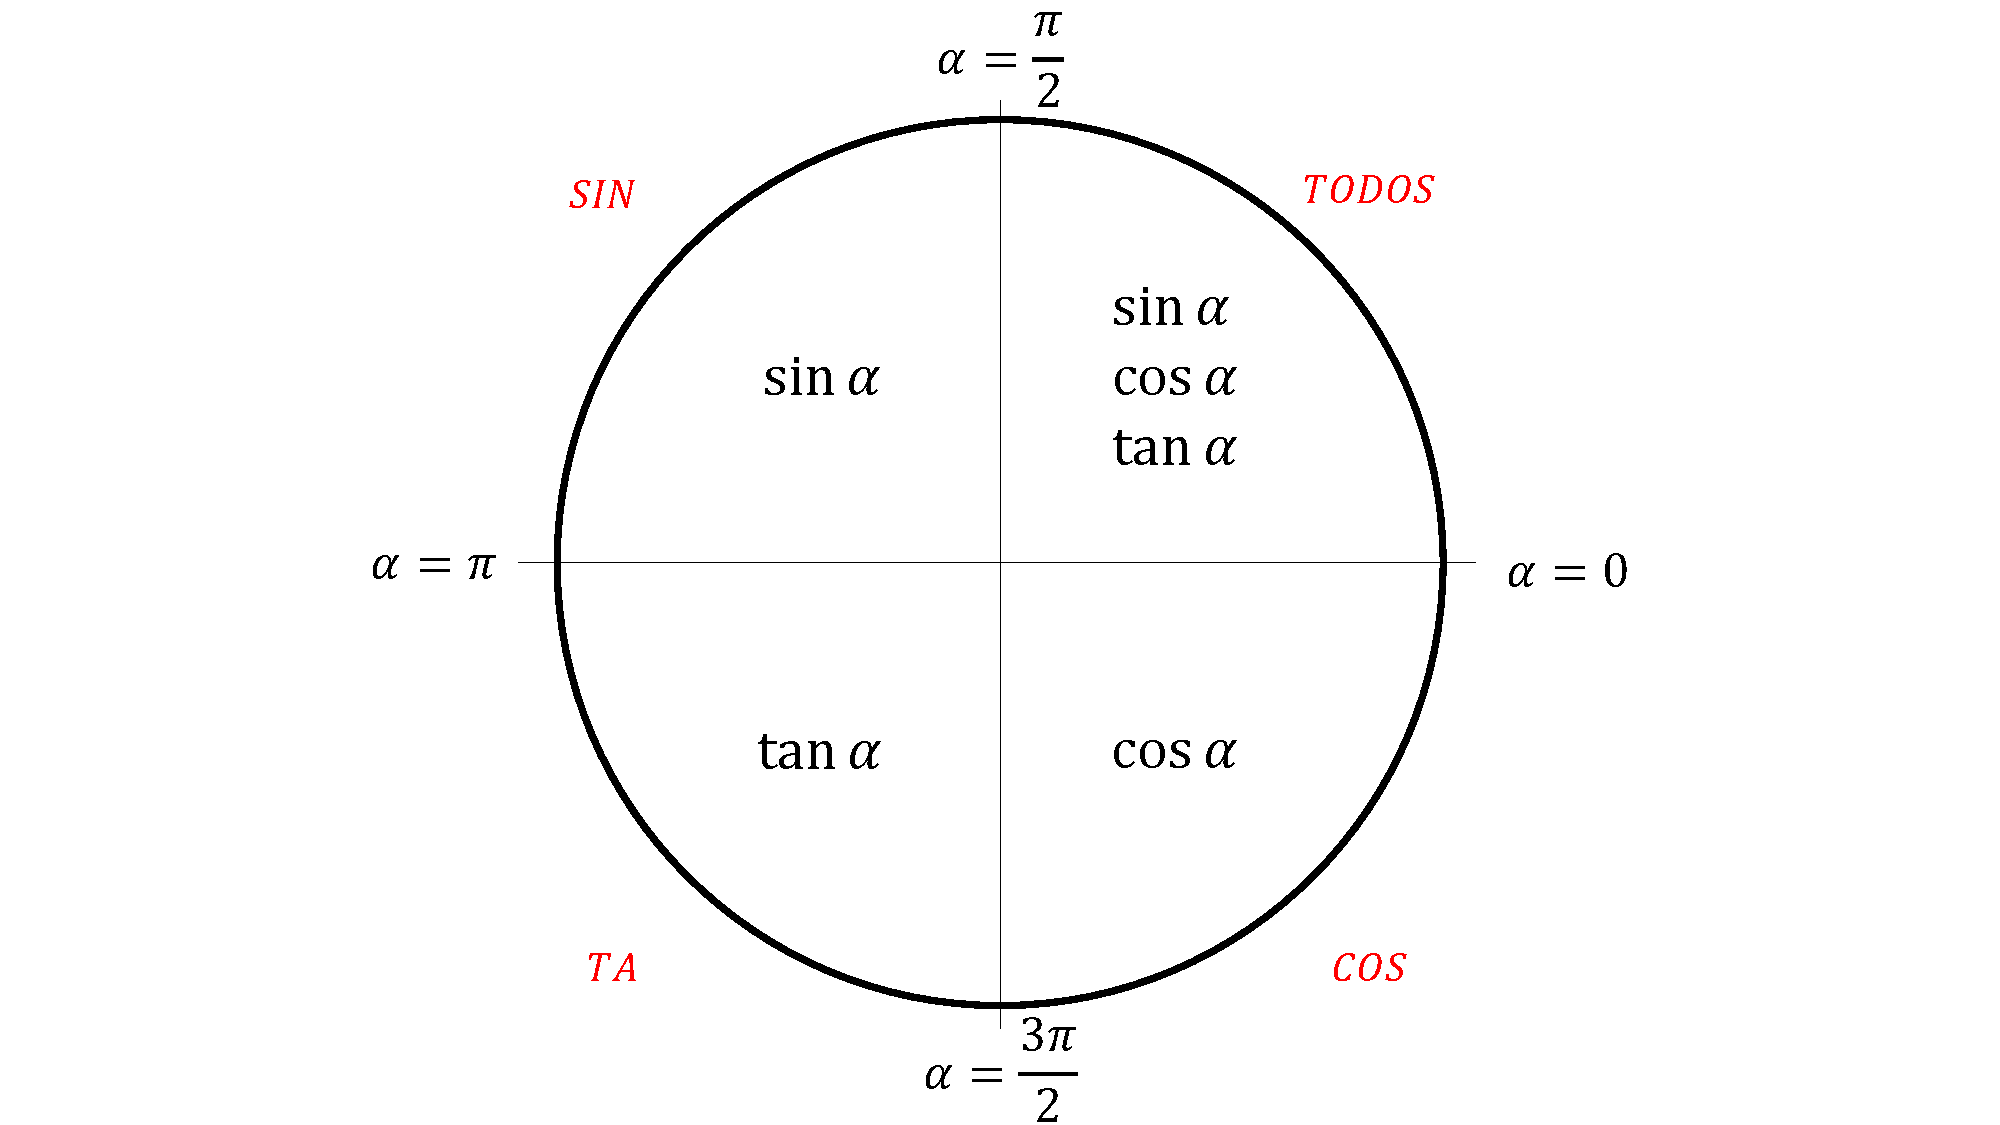
\includegraphics[scale=0.23]{Imágenes/resumen trig/todossintacos.pdf}}
    \end{picture}
    Ayudamemoria: las regiones en donde estas funciones son \\positivas pueden ser recordadas por la frase ``Todos sin ta-cos''
    
\item Ángulos negativos:\\
Es fácil observar que un ángulo negativo genera la misma proyección en el eje $x$, no así en el eje $y$, en donde la proyección se vuelve negativa. Es decir:

\begin{figure}[h!]
    \centering
    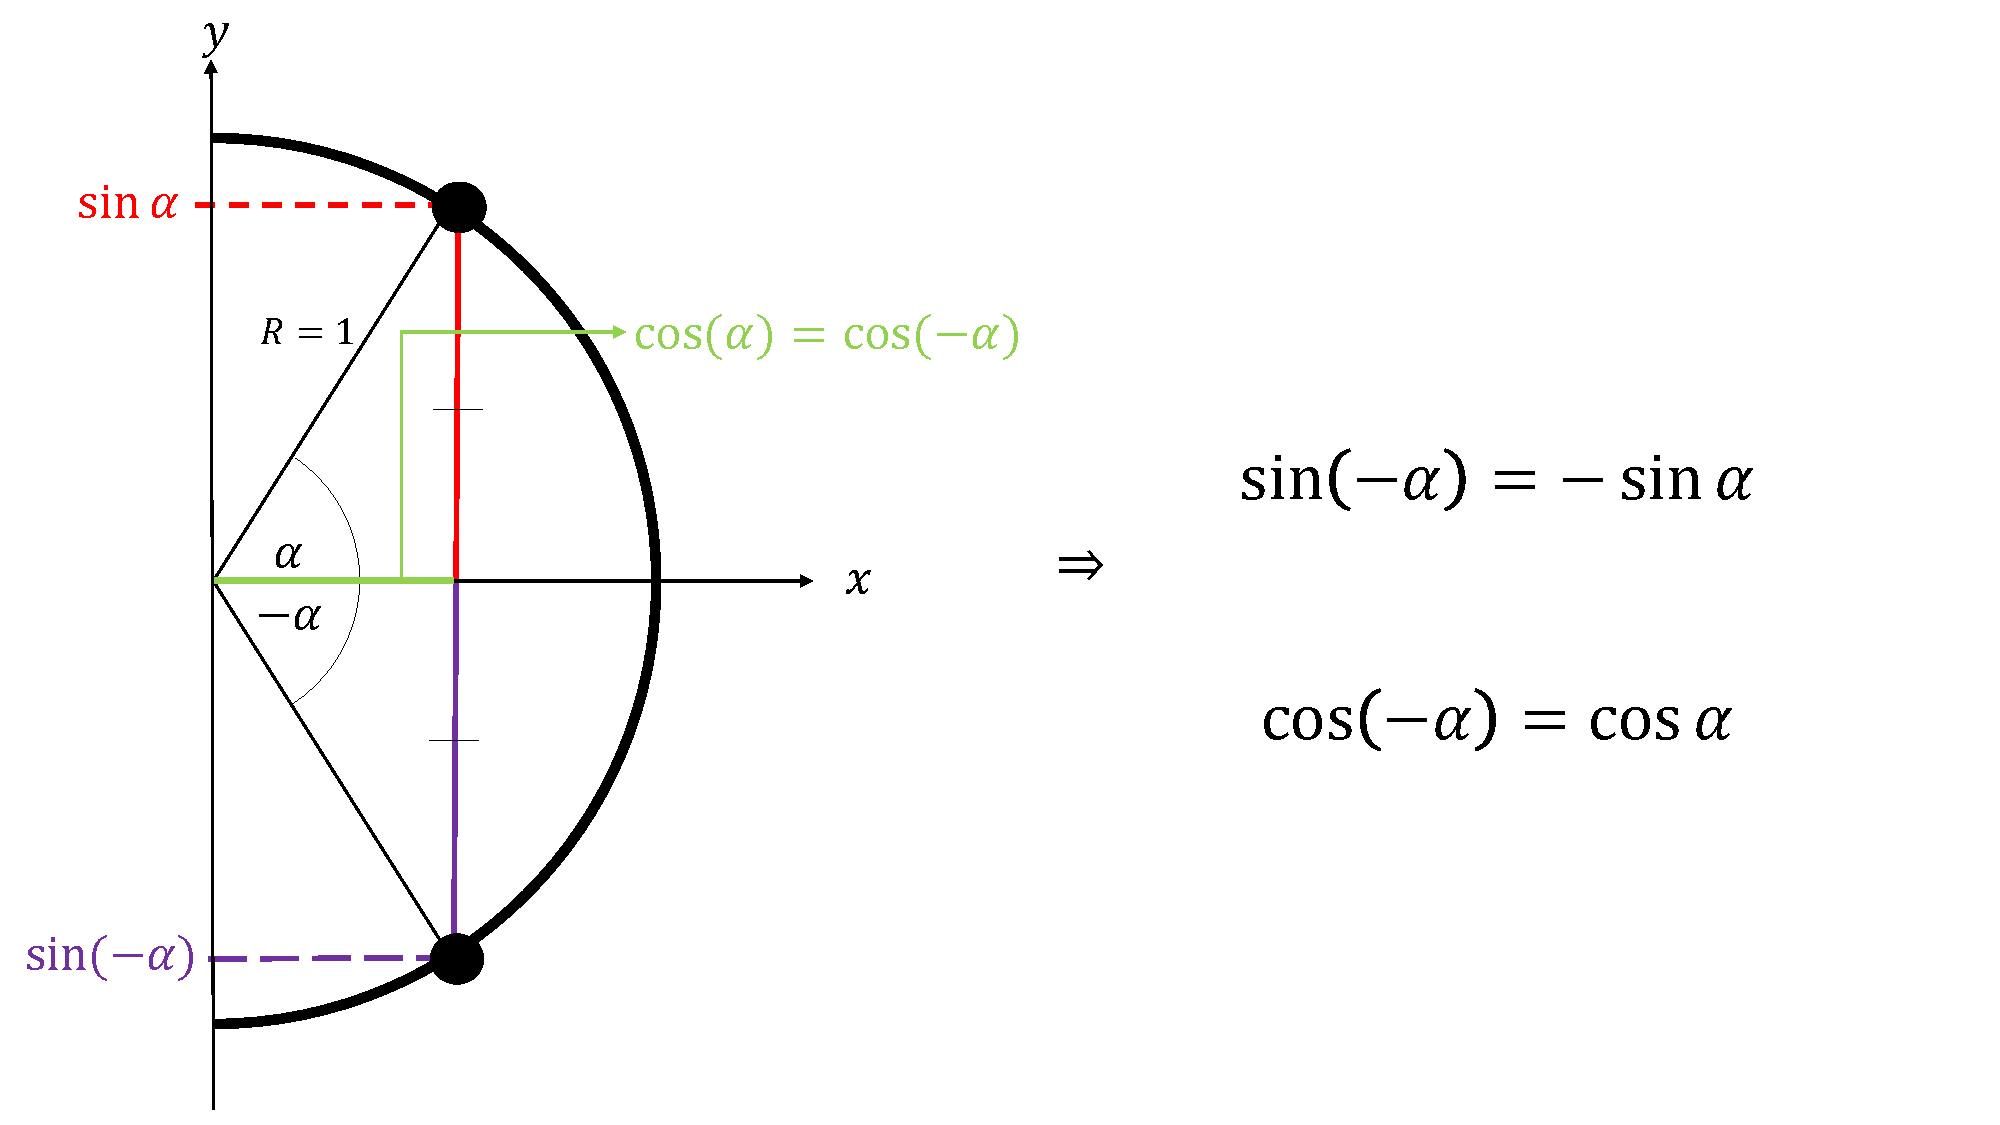
\includegraphics[scale=0.28]{Imágenes/resumen trig/menosalpha.pdf}
\end{figure}
Una función que cumpla $f(-x)=f(x)$ (como el coseno) se denomina \textbf{función par}, por otro lado, si cumple ${f(-x)=}~{-f(x)}$ (como el seno) se denomina \textbf{función impar} 
\end{itemize}

\section{Otras identidades importantes}
Las siguientes identidades serán de mucha utilidad y verán sus demostraciones en profundidad en Introducción al Cálculo

\begin{itemize}
    \item Suma de ángulos:
    \begin{itemize}
        \item $\sin(\alpha+\beta)=\sin\alpha\cos\beta+\sin\beta\cos\alpha$
        \item $\cos(\alpha+\beta)=\cos\alpha\cos\beta-\sin\alpha\sin\beta$
        \item La resta es aplicar paridad/imparidad de las funciones
    \end{itemize}
    
    \item Teorema del Seno y del Coseno: Para cualquier triángulo se cumplen las siguientes relaciones
    \begin{itemize}
        \item Teorema del Seno: $\cfrac{\sin\alpha}{a}=\cfrac{\sin\beta}{b}=\cfrac{\sin\gamma}{c}$
        \item Teorema del Coseno:\\
        viene a ser una extensión del Teorema de Pitágoras
        \begin{itemize}
            \item $a^2=b^2+c^2-2bc\cos\alpha$
            \item $b^2=a^2+c^2-2ac\cos\beta$
            \item $c^2=a^2+b^2-2ab\cos\gamma$
        \end{itemize}
            \begin{picture}(2,3)
        \put(330,20){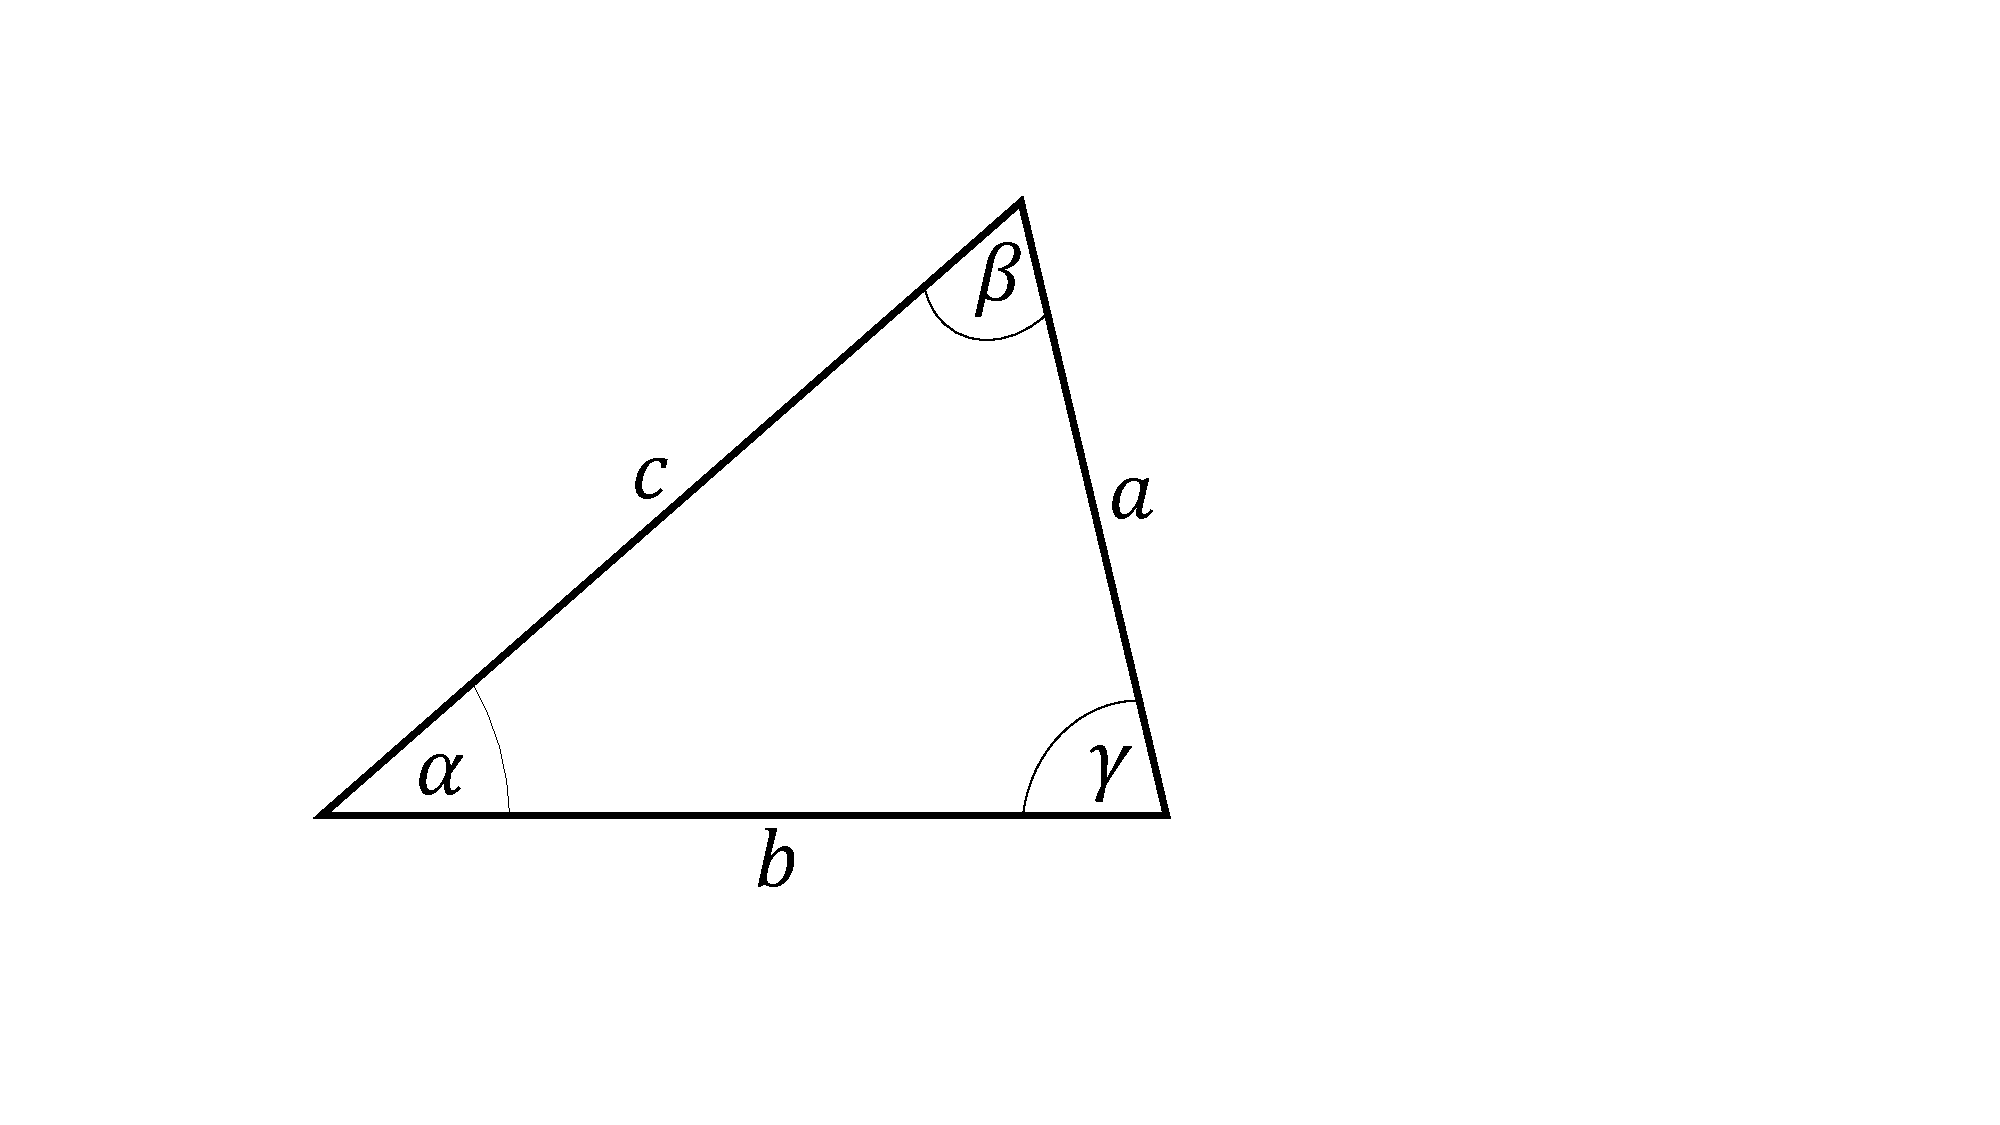
\includegraphics[scale=0.23]{Imágenes/resumen trig/acutang.pdf}}
    \end{picture}
    \end{itemize}
\end{itemize}

\subsection*{Tabla de valores de ángulos ``importantes''}

\begin{table}[h!]
    \centering
    \begin{tabular}{m{2em}||m{2em}|m{2em}|m{2em}|m{2em}|m{2em}|}
         $\alpha$ & $0$ & $\dfrac{\pi}{6}$ & $\dfrac{\pi}{4}$ & $\dfrac{\pi}{3}$ & $\dfrac{\pi}{2}$\\[2ex] \hline
         $\sin\alpha$ & $0$ & $\dfrac{1}{2}$ & $\dfrac{\sqrt{2}}{2}$ & $\dfrac{\sqrt{3}}{2}$ & $1$\\[3ex] 
         $\cos\alpha$ & $1$ & $\dfrac{\sqrt{3}}{2}$ & $\dfrac{\sqrt{2}}{2}$ & $\dfrac{1}{2}$ & $0$ \\[3ex] 
         $\tan\alpha$ & $0$ & $\dfrac{\sqrt{3}}{3}$ & $1$ & $\sqrt{3}$ & $\nexists$
    \end{tabular}
\end{table}
\begin{itemize}
    \item Ayudamemoria: notar que para el seno y el coseno la tabla se arma de la siguiente manera
    \begin{itemize}
        \item para el seno se completa con $0,1,2,3,4$ y para el coseno con $4,3,2,1,0$
        \item tomar raíz 
        \item dividir por 2
    \end{itemize}
\end{itemize}
\end{document}